\item A small bar $A$ resting on a smooth horizontal plane is attached by threads to a point $P$ (Fig. 1.34) and, by means of a weightless pulley, to a weight $B$ possessing the same mass as the bar itself.
    \begin{center}
        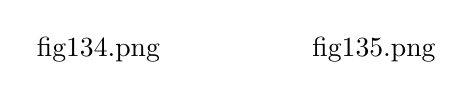
\begin{tikzpicture}
            \node at (0, 0) {{fig134.png}};
            \node at (3.5, 0) {{fig135.png}};
        \end{tikzpicture}
    \end{center}
Besides, the bar is also attached to a point $O$ by means of a light non-deformed spring of length $l_0 = 50 \text{ cm}$ and stiffness $k = 5 \frac{mg}{l_0}$, where $m$ is the mass of the bar. The thread $PA$ having been burned, the bar starts moving. Find its velocity at the moment when it is breaking off the plane.
    \begin{enumerate}
        \item Calculate the initial acceleration of the bar.
        \item Determine the velocity of the bar using the equation of motion.
    \end{enumerate}\begin{solution}
    \begin{center}
        \begin{tikzpicture}
            \pic at (0, 0) {frame=3cm};
        \end{tikzpicture}
    \end{center}
    
    \begin{align*}
        \intertext{When the thread \(PA\) is burnt, obviously the speed of the bars will be equal at any instant of time until it breaks off. Let \(\nu\) be the speed of each block and \(\theta\) be the angle, which the elongated spring makes with the vertical at the moment when the bar \(A\) breaks off the plane. At this stage the elongation in the spring is}
        \Delta l &= l_0 \sec \theta - l_0 = l_0 (\sec \theta - 1) \tag{1}\\
        \intertext{Since the problem is concerned with position and there are no forces other than conservative forces, the mechanical energy of the system (both bars + spring) in the field of gravity is conserved, i.e., \(\Delta T + \Delta U = 0\).}
        \intertext{So,}
        2 \left(\dfrac{1}{2}mv^2\right) + \dfrac{1}{2}k l_0^2 (\sec \theta - 1)^2 - mg l_0 \tan \theta &= 0 \tag{2}\\
        \intertext{From Newton's second law in projection form along vertical direction:}
        mg &= N + \kappa l_0 (\sec \theta - 1) \cos \theta\\
        \intertext{But, at the moment of break off, \(N = 0\).}
        \kappa l_0 (\sec \theta - 1) \cos \theta &= mg\\
        \intertext{Hence,}
        \cos \theta &= \dfrac{\kappa l_0 - mg}{\kappa l_0} \tag{3}\\
        \intertext{Taking \(\kappa = \dfrac{5mg}{l_0}\), simultaneous solution of Eqs. (2) and (3) yields}
        v &= \sqrt{\dfrac{19g l_0}{32}} \approx 1.7\, \text{m/s}
    \end{align*}
\end{solution}